What you need to follow along:

\begin{itemize}
    \item HDF5 library source code~\cite{libhdf52023}
    \item GCC~\cite{gcc2023} (compile stuff w/ \texttt{-g})
    \item Valgrind~\cite{valgrind2023}
    \item KCachegrind~\cite{kcachegrind2023}
    \item CMake~\cite{cmake2023}
    \item A clone of the GitHub repository~\cite{hdf5-tourist}, which contains the code samples
\end{itemize}

\begin{minted}{shell}
# run the program with callgrind; generates a file callgrind.out.XYZUV
valgrind --tool=callgrind ./executable

# open profile.callgrind with kcachegrind
kcachegrind callgrind.out.XYZUV
\end{minted}

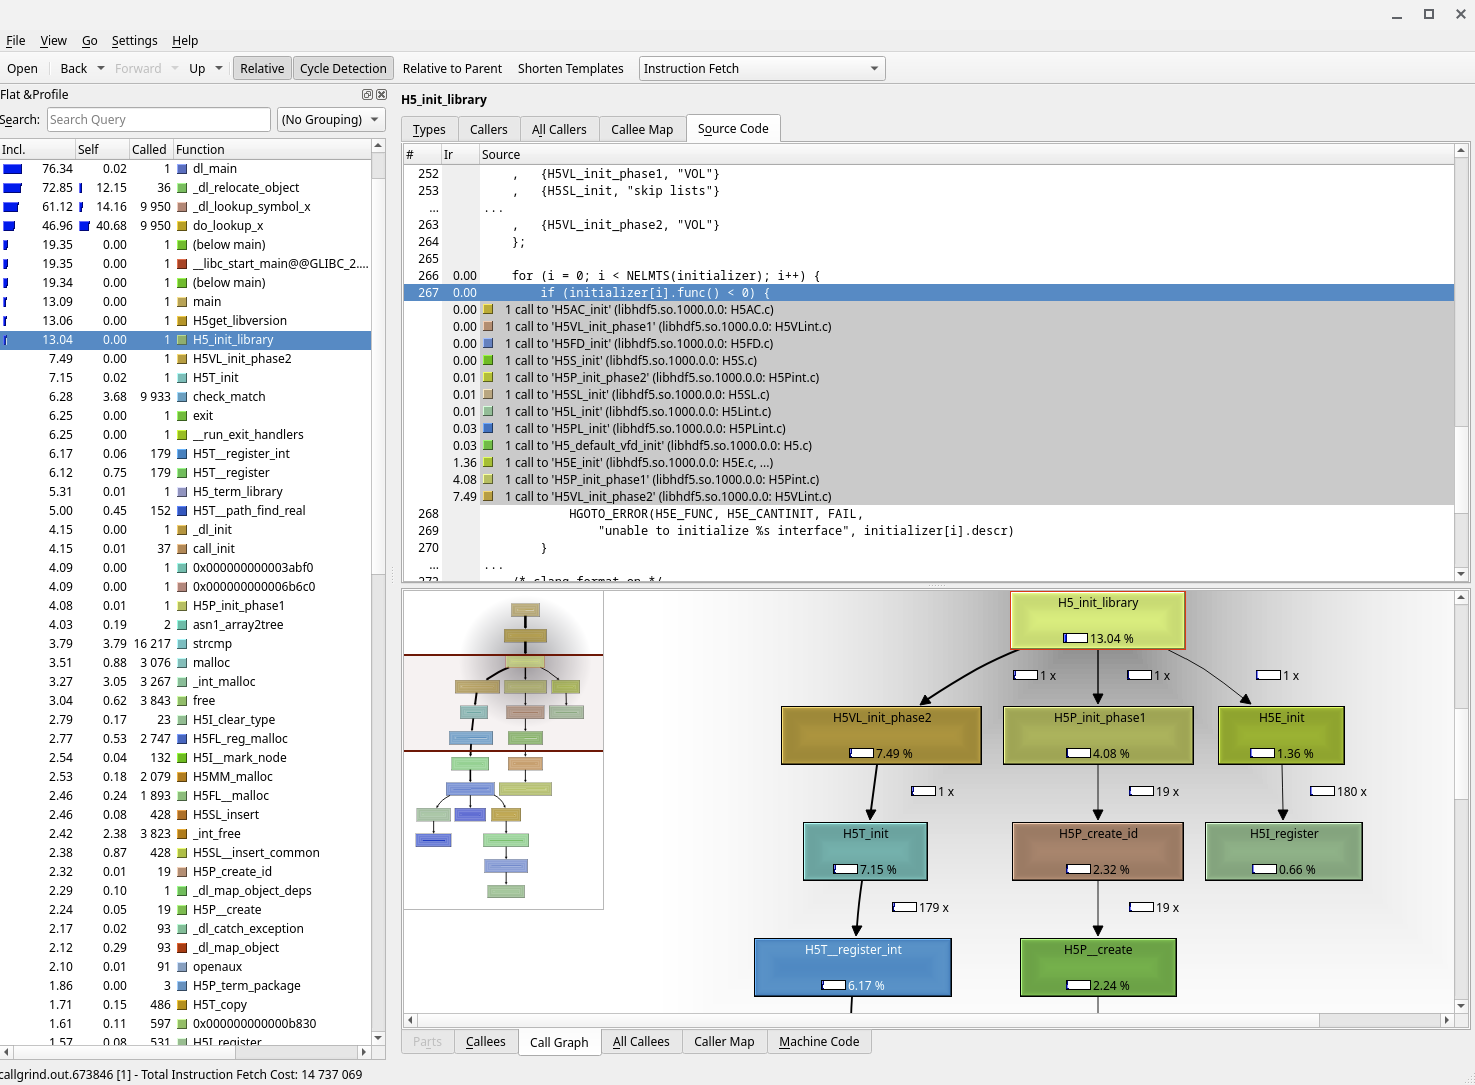
\includegraphics[scale=0.3]{images/kcachegrind.png}

Ease of navigation\ldots, but don't be fooled by pictures! You must look at the code.

\begin{figure}
\centering
\caption{Caption}
\label{fig:label1}
\begin{minted}[linenos]{C}
    ...
    struct {
        herr_t (*func)(void);
        const char *descr;
    } initializer[] = {
        {H5E_init, "error"}
    ,   {H5VL_init_phase1, "VOL"}
    ,   {H5SL_init, "skip lists"}
    ,   {H5FD_init, "VFD"}
    ,   {H5_default_vfd_init, "default VFD"}
    ,   {H5P_init_phase1, "property list"}
    ,   {H5AC_init, "metadata caching"}
    ,   {H5L_init, "link"}
    ,   {H5S_init, "dataspace"}
    ,   {H5PL_init, "plugins"}
    /* Finish initializing interfaces that depend on the interfaces above */
    ,   {H5P_init_phase2, "property list"}
    ,   {H5VL_init_phase2, "VOL"}
    };

    for (i = 0; i < NELMTS(initializer); i++) {
        if (initializer[i].func() < 0) {
            HGOTO_ERROR(H5E_FUNC, H5E_CANTINIT, FAIL,
                "unable to initialize %s interface", initializer[i].descr)
        }
    }
    ...
\end{minted}
\end{figure}